\documentclass[a4paper,10.5pt]{ltjsarticle}
\usepackage{graphicx}
\usepackage{luatexja-fontspec}
\usepackage{caption}
\usepackage{amsmath,amssymb,bm,braket}
\usepackage[english]{babel}
%\usepackage{gnuplot-lua-tikz}
\usepackage[top=10truemm,bottom=15truemm,left=10truemm,right=10truemm]{geometry}
\usepackage{array}
\usepackage{upgreek}
\usepackage{fancyhdr}
\renewcommand{\refname}{}
\usepackage{listings,jvlisting}
\usepackage{tikz}
\usepackage[version=3]{mhchem}
\usetikzlibrary{external}
\tikzexternalize
\lstset{
  basicstyle={\ttfamily},
  identifierstyle={\small},
  commentstyle={\smallitshape},
  keywordstyle={\small\bfseries},
  ndkeywordstyle={\small},
  stringstyle={\small\ttfamily},
  frame={tb},
  breaklines=true,
  columns=[l]{fullflexible},
  numbers=left,
  xrightmargin=0pt,
  xleftmargin=3pt,
  numberstyle={\scriptsize},
  stepnumber=1,
  numbersep=1pt,
  lineskip=-0.5ex
}
\captionsetup[figure]{format=plain, labelformat=simple, labelsep=quad,labelfont=bf}
\captionsetup[table]{format=plain, labelformat=simple, labelsep=quad,labelfont=bf}
\parindent = 0pt
\setmainjfont[BoldFont=HGSMinchoE]{MSMincho}
%[BoldFont=HGSMinchoE]{MSMincho}[BoldFont=HiraMinProN-W6]{HiraMinPro-W3}
\begin{document}
\centerline{\Large     z軸方向移動の問題について}
\centerline{}
 3D lattice surgeryでz方向の移動は、pipeline内のqubit同士でCNOTをかけないと行けないため、あまりしたくない。looped pipelineの論文ではCZゲートをかけるのに100nsかかると仮定されている。そこで、CZゲートかける時間が1回だけで済むようなpipelineの配置を考える。pipelineの性質として、最上階の平面と最下階の平面は隣接しているためFigure 1のような移動が可能である。\\
\begin{figure}[h]
  \centering
  \includegraphics[scale=0.6]{figure1.eps}
  \vspace{-20pt}\caption{}
\end{figure}\\
それぞれのpipeline内のqubitの種類を変えることによってFigure 2のような構造を作ることができる。左から6番目のpipelineでは、黒とピンクが隣り合っているから、floor 4からfloor 0へのワープが可能。7番目のpipelineでも同様に、黒と緑が隣り合っているからfloor3からfloor0へのワープが可能。8番目についても同じ。
\begin{figure}[h]
  \centering
  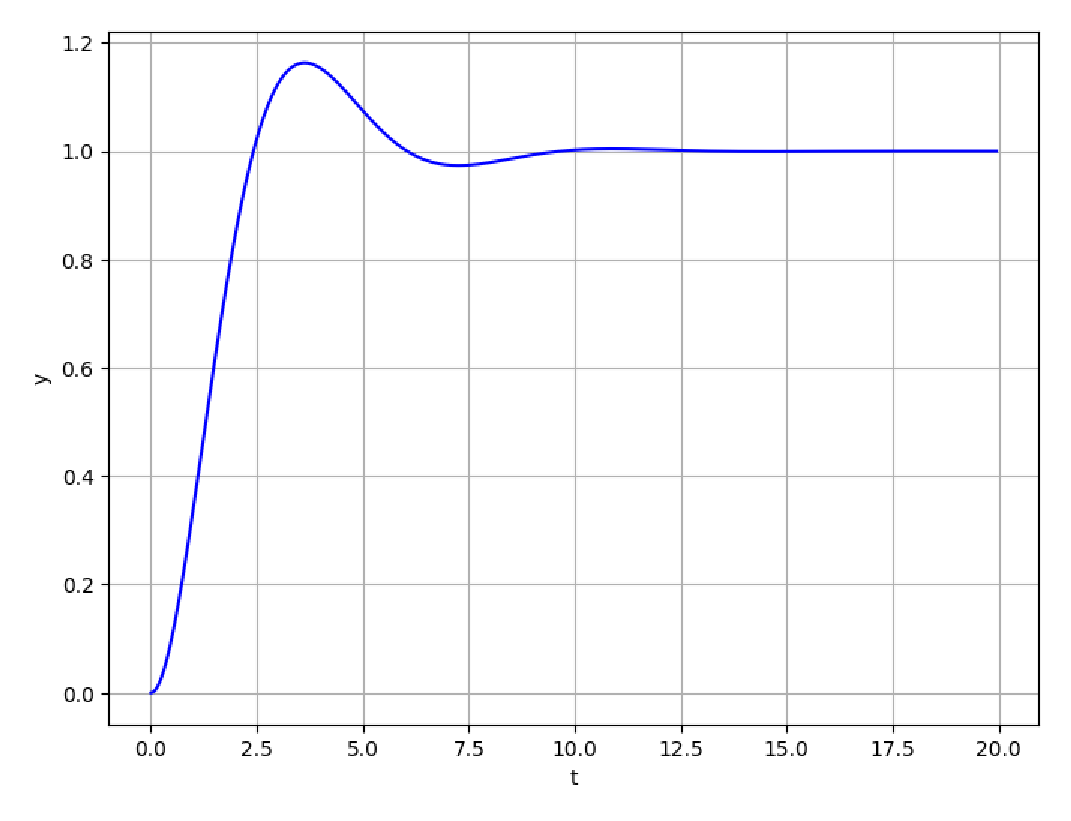
\includegraphics[scale=0.5]{figure2.eps}
  \vspace{-20pt}\caption{}
\end{figure}
\clearpage
floor 5にスタート地点(S)、floor 2にゴール地点(G)を置き、これらをlattice surgeryでつなげるとすると、Figure 3のようにすればよい。まず、Sから経路を伸ばすと同時にGから経路を伸ばす。そして、floor 5→floor 0とfloor 2→floor 0のCZは同時にかける。最後にfloor 0上で2つの経路をつなぐ。このようにすれば、スタート地点とゴール地点がどの階にあったとしても、CZの時間を1回だけ待つだけでつなぐことができる。\\
\begin{figure}[h]
  \centering
  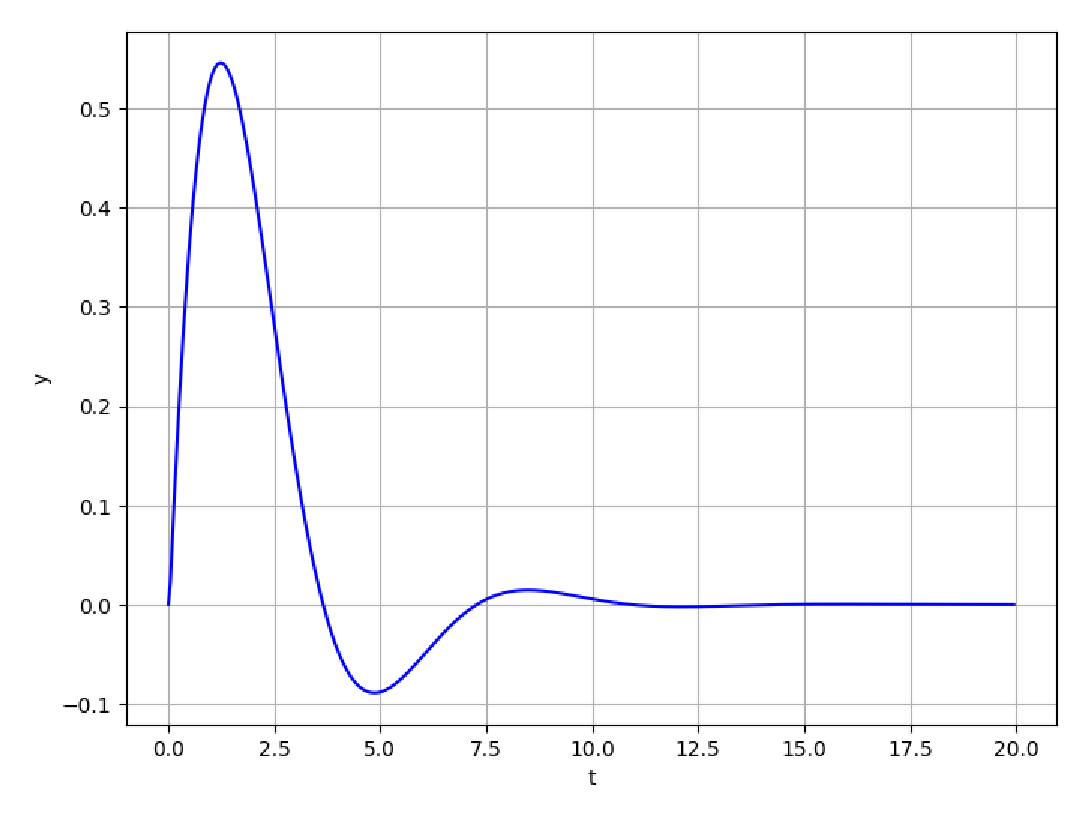
\includegraphics[scale=0.6]{figure3.eps}
  \vspace{0pt}\caption{}
\end{figure}\\
pipeline内のqubitが2個もしくは3個の部分をところどころに配置しておけば、1回のz軸方向の移動でどの階にも行けるが、どの色のqubitを2個または3個選ぶと最適であるかはかなり複雑。このような問題は多角形の辺と対角線上での一筆書きの問題に落とし込むことができる。例えば、0階から4階までしかない構造を考えるとFigure 4のようになる。\\
\begin{figure}[h]
  \hspace{-80pt}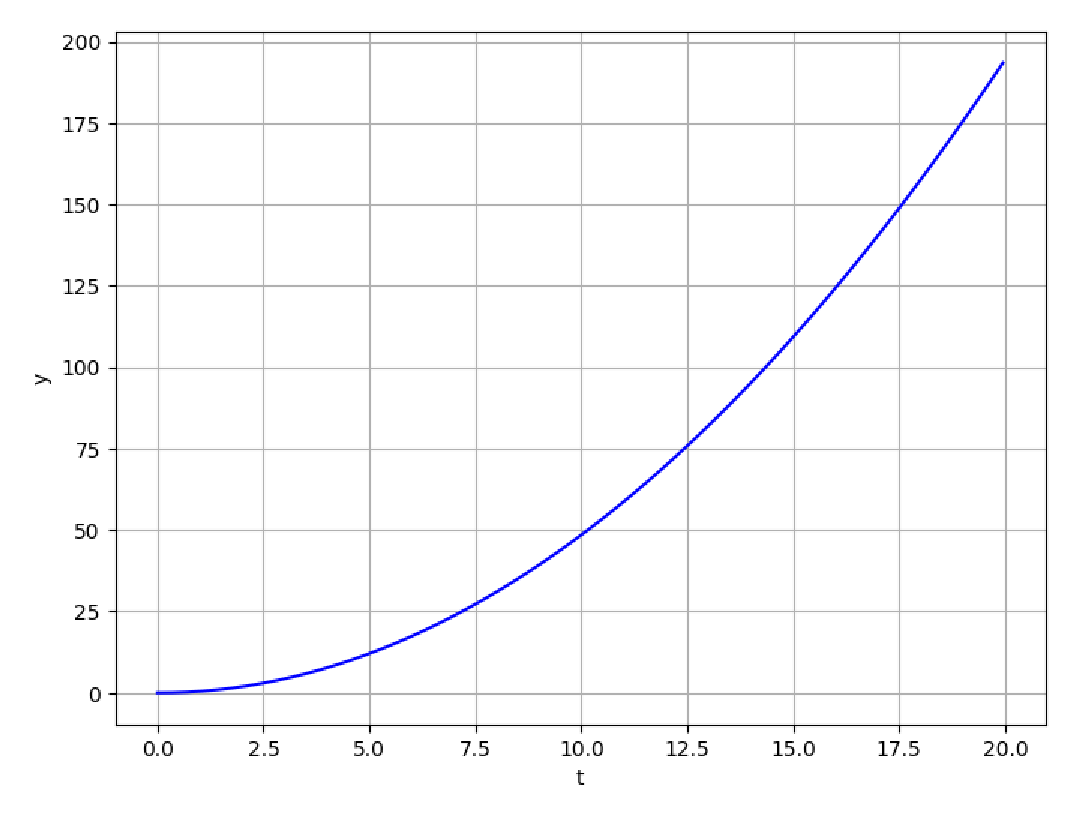
\includegraphics[scale=0.55]{figure4.eps}
  \vspace{-30pt}\caption{}
\end{figure}\\
Figure 4の右側の五角形の実線は左側の隣り合う階(floor 4とfloor 0も隣り合う)を表している。今、どの階にいても他のすべての階に1回だけのz軸方向の移動だけで行けるようにするためには、五角形の破線で繋がれている点同士を実線でつなぐようなpipeline必要である。例えば、Figure 5右側のような一筆書きで破線をなぞる。
\clearpage
\begin{figure}[h]
  \hspace{-80pt}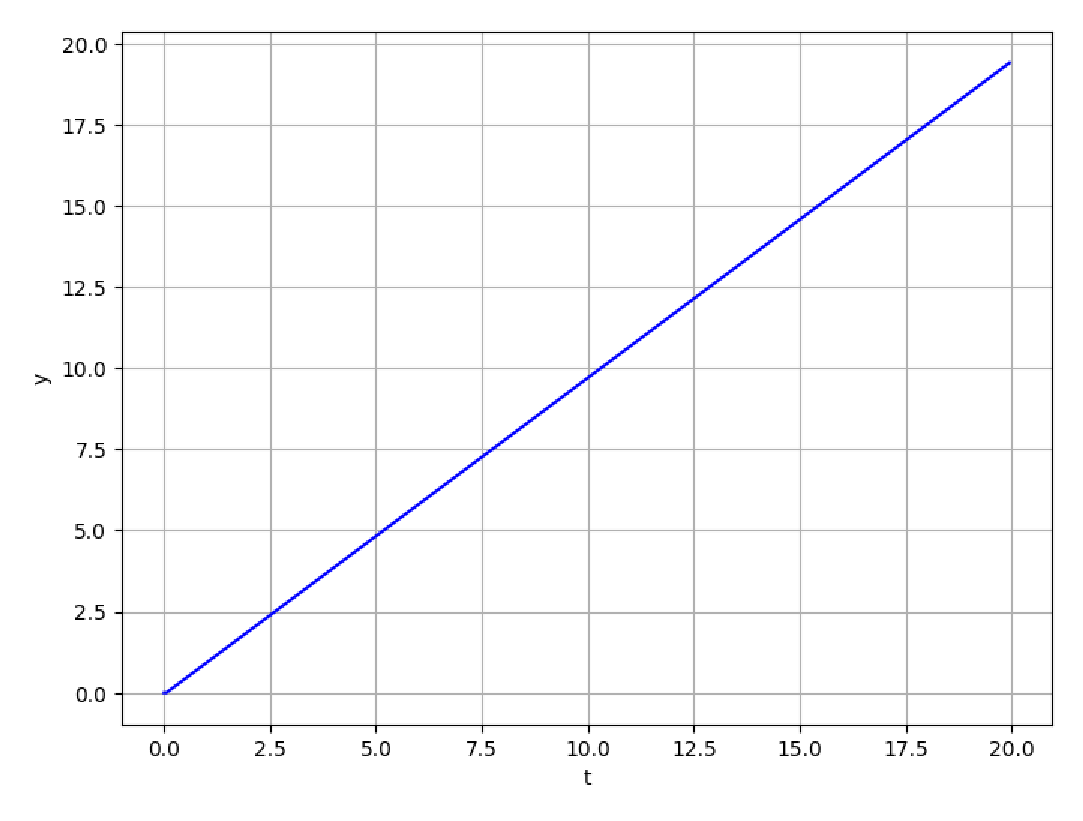
\includegraphics[scale=0.55]{figure5.eps}
  \vspace{-15pt}\caption{}
\end{figure}\\
このようにすると、Figure 5左側のような1種類のpipelineを追加することで、どの階にいたとしても他のすべての階に1回のz軸方向の移動でいける。ただし、2種類のpipelineの同期の難しさについては全く考慮していない。なので、おそらくFigure 6のようにするほうが同期は簡単だと思われる。\\
\vspace{-70pt}\begin{figure}[h]
  \hspace{-70pt}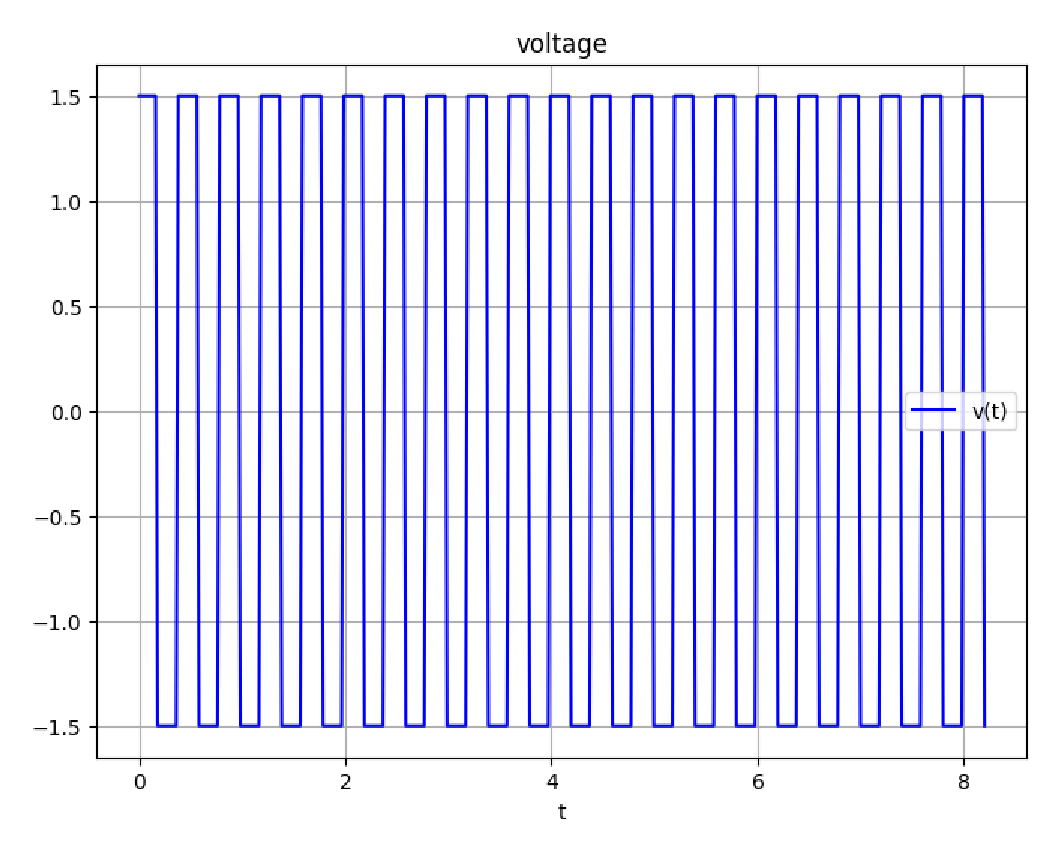
\includegraphics[scale=0.4]{figure6.eps}
  \vspace{-15pt}\caption{}
\end{figure}\\


\end{document}
